\chapter{Le développement de jeux vidéos}
 
 
\section{Les étapes de création}
%Conférence Ubisoft a l'UQAM
La liste des étapes de création est non exhaustive et est à titre informatif afin de représenter les étapes dans un environnement de développement particulier présenté par Mathieu Nayrolles lors d'une présentation réalisée dans le cadre d'un séminaire au LATECE (Laboratoire de recherche sur les technologies du commerce électronique) de l'UQAM.
\begin{figure}[H]
    \centering
    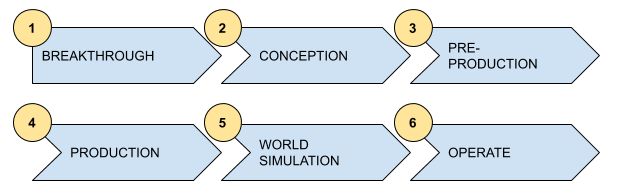
\includegraphics[width=14cm]{10_img/production_stages.png} 
    \caption{Étapes de création d'un jeu vidéo}
\end{figure}
\subsection{Breakthrough}
Une étape de Breakthrough est optionnelle et peut être à l'origine d'un nouveau jeu vidéo mais également d'une nouvelle technologie dans le domaine
Par exemple :
\begin{itemize}
    \item Une percée technologique. Ex : Google lance Stavia une plateforme en ligne de jeux vidéos sous forme de catalogue et jouable à 100\% en ligne sans installation en local
    \item Une percée de Gameplay. Ex : naissance du mode Battle Royale
\end{itemize}

\subsection{Conception}
Un document de concept est prototypé afin de définir l'environnement, la faisabilité et l'intérêt commercial du jeu. C'est durant cette étape que les game designer définissent l'univers, les mécaniques et le déroulement du jeu vidéo en question. Cette étape est majoritairement gérée par les Game Designers appuyés par les équipes des autres corps de métier.

\subsection{Pre-production}
Durant cette étape des prototypes sont développés afin de créer une partie minimale du jeu. Cela permet d'avoir un aperçu de ce que pourrait donner le jeu final en fonction des documents de concepts créés durant l'étape de conception dans un environnement réduit. C'est une coupe verticale de tout le système et qui permet de réfléchir à des ajustements possibles des documents de conception afin de les rendre plus efficaces. Une fois le design bien définit, le prototype au plus proche de ce que donnerait le jeu final et la faisabilité du projet confirmée, il est alors possible de rechercher les financements et les ressources nécessaires à la production. Cette étape est gérée par tous les corps de métier dans un studio de développement, tous les aspects du jeu devant être représentés afin de montrer tout le potentiel du prototype.

\subsection{Production}
Une fois les fonds levés et les ressources humaines attitrées au projet il est alors possible de procéder à la production du jeu vidéo. Tous les corps de métier sont alors représentés et le jeu est développé sous tous ses aspects et dans son intégralité. Selon les méthodes de gestion de projet le projet avance sous forme d'itérations afin de vérifier que le développement respecte bien les concepts du jeu vidéo et suive bien le parcours définis dans les documents de conception. Durant cette étape des modifications peuvent être apportées en fonction des problématiques rencontrées ou des contraintes du projet. Généralement durant cette étape le marketing et la publicité autour du jeu commence à prendre place afin de prévenir le public et d'estimer l'impact que peut avoir le jeu.

\subsection{Simulation}
Lors de cette étape tous les éléments du jeu sont testés et passés au crible. On vérifie que les éléments de jeu soient correctement modélisés, que les sons correspondent bien aux éléments, que les personnages soient bien comme décris dans les documents de conception... Plusieurs questions se posent à ce moment là. Est-ce que les éléments interagissent bien entre eux ? Est-ce que l'univers de jeu est cohérent de bout en bout ? Est-ce que le gameplay est fluide et intuitif ? Est-ce que l'environnement de jeu est réellement comme le décrit le game designer ? Est-ce que la bande sonore ou la modélisation graphique génère bien l'émotion attendue chez le joueur ?

\subsection{Distribution et fonctionnement}
Le jeu est maintenant produit et commercialisé. Une quantité importante de données est ainsi générée, des bugs peuvent être remontés et corrigés dans des cas de figure particuliers ou inédits non couverts par l'étape de World Simulation. Des ajustements mineurs peuvent être fais en fonction des besoins ou des demandes des joueurs. Le jeu prend alors toute sa dimension et toute sa vie à travers les joueurs.

\subsection{Nouveau contenu}
Une fois le jeu bien en place et les étapes de corrections et ajustements passées et en fonction de la popularité du jeu il est possible alors d'intégrer du nouveau contenu au jeu en question en repassant par les étapes précédentes afin d'intégrer le nouveau contenu dans le jeu sous forme de \gls{dlc}.

\subsection{Conclusion}
Le contenu de ce travail de recherche se concentre sur l'établissement d'un modèle afin de faciliter la rédaction d'un Game Design Document, nous nous concentrerons donc sur l'étape de Conception d'un jeu vidéo. C'est durant cette étape que les documents de conception prennent forme et deviennent le support sur lequel repose l'intégralité du développement du jeu vidéo comme une bible devant contenir toutes les informations nécessaires au bon déroulement du projet et à sa cohérence de bout en bout.



\section{Exploitation et exploration}
\subsection{Exploitation}
L'exploitation dans le développement de jeux vidéos est une part importante du travail d'un studio de développement. De nombreux jeux vidéos récents sont basés sur de l'exploitation de jeux précédents autant au niveau du gameplay qu'au niveau des concepts fondamentaux de jeux précédents. C'est le cas de grosses productions de franchises comme les jeux de EA sports (FIFA, NHL, NBA Live, Madden), les jeux d'action role-play de FromSoftware (série des Dark Souls), les jeux d'action aventure de Rockstar (série des GTA) ou les jeux de simulation de Maxi/EA Games (série les Sims). Le travail d'exploitation consiste à produire une suite ou un nouveau jeu en utilisant des technologies (moteur, plateformes, etc) ou un gameplay déjà existant afin de recréer un jeu ou produire du contenu additionnel. Ceci peut être fait dans un but de fidéliser une clientèle déjà existante en ajoutant du contenu additionnel à un jeu, à offrir une expérience similaire avec des technologie plus récentes (ex : FIFA) ou à offrir une suite à un jeu ayant déjà connu du succès (ex : Dark Souls).

\subsection{Exploration}
L'innovation dans le monde du de jeux vidéos est essentielle au développement de nouveaux concepts de gameplay mais également de nouvelles technologies. C'est pour cela qu'une grande partie de l'investissement en temps et en argent du monde du développement de jeux vidéos se situe dans des processus exploratoires et la recherche et développement. De la recherche de nouveaux concepts de jeux, de nouveaux types de gameplay, de nouvelles technologies à intégrer ou de la création de nouveaux moteurs de jeux, l'exploration est devenu un facteur essentiel au domaine du jeu vidéo et à son expansion.


\subsection{Conclusion}
Il est nécessaire, pour les studios de développement de jeux vidéos, de trouver le bon équilibre entre exploitation et exploration afin d'offrir aux clients des articles de qualité et attractifs. Cet équilibre est précaire et il est difficile pour un studio de développement d'investir sur les deux domaines à la fois en particulier en fonction de la taille de celui-ci. Dans leur article Parmentier et al \cite{ParmentierGuy2009Iecd} explorent la capacité des studios à concilier ces deux activités en expliquant les enjeux de chacune d'entre elles et leur importance dans le domaine.



\section{Les moteurs de jeux}
Un moteur de jeu (Game engine) est le plus souvent une suite logicielle contenant un framework de mécaniques de jeu permettant d'accélérer le développement d'un jeu vidéo. Il peut inclure une ou plusieures facettes du développement du jeu allant de la physique, aux graphismes, aux sons, aux calculs, à la gestion des périphériques d'entrée/sortie jusqu'à la gestion automatique de l'intelligence artificielle. Voici une liste des moteurs de jeu les plus connus accompagnés des jeux qui en font usage : 
\begin{itemize}
    \item Unreal Engine développé par Epic Games : Fortnite, Outlast 2, Dragon Ball Fighter Z, Days Gone.
    \item Unity dévelooppé par Unity Technologies : 7 Days to Die, Cuphead, Ori and the Blind Forest, Pokemon Go.
    \item CryEngine développé par Crytek : Far Cry, Crysis 3, Deceit, Mavericks.
    \item Frostbite développé par Dice (EA) : Battlefield V, Anthem, FIFA, Need for Speed.
\end{itemize}

Chaque moteur de jeu présente des avantages et des inconvénients en fonction du type de jeu que l'on souhaite développer, même si certains contiennent des technologies plus axées sur un type de jeu en particulier. L'innovation dans le domaine du moteur de jeu est essentielle au développement de nouveaux jeux vidéos car c'est avec ces outils qu'il est possible de créer ou mettre en place plus rapidement des éléments plus récents de l'innovation comme des graphismes plus réalistes ou détaillés ainsi que des intelligences artificielles plus évoluées.

\section{Les types de Gameplay}
L'exploration peut également consister en la création d'un nouveau mécanisme de gameplay. Ce genre d'innovation est plus facilement repérable par le joueur et plus marquante concernant l'expérience de jeu. Voici une liste non exhaustive des principaux types de gameplay présents dans le jeu vidéo :
\begin{itemize}
    \item MMORPG (Massive Multiplayer Online Role-Playing Games) : Jeu massivement multijoueur en ligne mettant en scène un jeu de role play avec différents objectifs à remplir (leveling, histoire principale/secondaire, développement social pour atteindre ces objectifs sous forme de guilde...) (ex : World of WarCraft, Black Desert Online)
    \item Survival : le joueur doit survivre aux événements présents dans le jeu, il peut devoir subvenir à des besoins vitaux, construire de nouveau objets, ou survivre aux autres joueurs présents (ex : Rust, Ark)
    \item Plateformes : un joueur contrôle un personnage qui se déplace dans un environnement de plateformes et doit avancer tout au long du niveau pour le finir (ex : Mario, Donkey Kong)
    \item Simulation de vie : Le joueur gère un ou plusieurs personnages, ou même une ville et simule un environnement de vie plus ou moins réaliste en fonction des objectifs du jeu (ex : Les Sims, SimCity)
    \item FPS (First Personnal Shooter) : le joueur est seul ou en équipe et doit battre les ennemis (IA ou autres joueurs) à l'aide d'armes et d'équipements de combat (ex : Call of Duty, Halo)
    \item Beat-em up : Le joueur fait face à des vagues d'ennemis toujours plus fortes (ex : Bayonnetta, God of War)
    \item RTS (Real Time Strategy) : Des joueurs se font fasse dans un jeu ou la gestion d'économie, de troupes et de population est omniprésente afin de battre les autres (Age of Empire, Starcraft)
    \item 4x : proche du RTS ce type de gameplay se base sur une gestion pointue de ressources et de population afin de pouvoir battre les autres joueurs sous différents aspects et avec différents objectifs de victoire (population max, évolution de la société, critères fininanciers...) (ex : Civilization, Stellaris)
    \item MOBA (Multiplayer Online Battle Arena) : C'est un type de gameplay ou le jeu d'action rencontre le RTS. Plusieurs (généralement deux) équipes de joueurs sont téléportées sur une carte, chaque joueur contrôle un personnage et les joueurs doivent détruire la base de l'équipe adverse. (ex : League of Legends, DOTA)
    \item Battle Royal : Plusieurs dizaines de joueurs sont parachutés sur une carte ou ils trouvent des armes et doivent s'entretuer. le dernier vivant est déclaré vainqueur. (ex : Fortnite, PUBG)
\end{itemize}

Ces types de gameplay se renouvellent régulièrement en fonction de l'attente des joueurs, en fonction de modes de jeu créés pour des jeux déjà existants ou en alliant plusieurs types de gameplay et en les adaptant afin d'en créer un nouveau. Ces types de gameplay sont classifiés en fonction du type de monde, des objectifs de jeu, des actions nécessaires... Dans leur article \cite{HeintzStephanie2015TGGM} essaient de mettre en place une cartographie des genres afin de classifier les différents types de jeux en se basant sur des caractéristiques précises des jeux et de leur gameplay. Cependant il est difficile d'arriver à classifier tous les jeux tellement les genres sont nombreux et entrecoupés c'est pour cela que la plupart des jeux sont classifiés dans des catégories relativement larges et sont différenciés par des caractéristiques différentes ensuite.



\section{Travail de recherche}
De nombreux challenges se rejoignent dans le développement de jeux vidéos et les outils et méthodes pour y parvenir sont déjà nombreux. Cependant il devient de plus en plus important dans ce secteur de chercher les méthodes possibles afin d'accélérer le développement sans pour autant impacter la qualité du contenu final. Les phases de Breakthrough et de Pré-conception sont essentielles à la création de nouveaux jeux vidéos, cependant plusieurs parties de ces étapes pourraient être accélérées afin de permettre l'élaboration d'un prototype plus rapidement. La phase de recherche des mécaniques de jeux et des objets le contenant est une phase importante. Un Game Designer se doit d'être précis et concis dans ses recherches et ses communications afin de communiquer un maximum d'informationsin de pouvoir dédier plus de temps à l'exploration, à la recherche artistique et au développement d'un prototype en Dans ce mémoire va être présenté un profil UML composé de stéréotypes qui permettra d'outiller  facilitant la documentation et la rédaction des documents descriptifs du jeu vidéo en cours d'élaboration
 


\begin{comment}
\section{Les métiers du développement de jeux vidéos}
\subsection{Les types de métiers}
\subsection{Les outils généraux}
\subsection{Les outils spécifiques}
\subsection{La difficulté de coordonner les travaux}
\end{comment}

